\documentclass[final]{beamer}

% ====================
% Packages
% ====================

\usepackage[T1]{fontenc}
 \usepackage[utf8]{luainputenc}
\usepackage{lmodern}
\usepackage[size=custom,width=297,height=210,scale=3.2]{beamerposter} % A4: 297mm x 210mm
\usetheme{gemini}
\usecolortheme{utb}
\usepackage{graphicx}
\usepackage{booktabs}
\usepackage{tikz}
\usepackage{pgfplots}
\pgfplotsset{compat=1.14}
\usepackage{anyfontsize}

% ====================
% Lengths
% ====================

% If you have N columns, choose \sepwidth and \colwidth such that
% (N+1)*\sepwidth + N*\colwidth = \paperwidth
\newlength{\sepwidth}
\newlength{\colwidth}
\setlength{\sepwidth}{0.025\paperwidth}
\setlength{\colwidth}{0.3\paperwidth}

\newcommand{\separatorcolumn}{\begin{column}{\sepwidth}\end{column}}

% ====================
% Title
% ====================

\title{\resizebox{\textwidth}{!}{Automatic Assessment of Tasks in the Course Programming Network Applications}}

\author{Author: \textbf{Ing. Martin Krčma}, Supervisor: \textbf{Ing. Tomáš Dulík, Ph.D.}}

\institute[shortinst]{Tomas Bata University in Zlin - Faculty of Applied Informatics} 

% ====================
% Footer (optional)
% ====================

\footercontent{
  \href{https://github.com/0xMartin}{Github: \textbf{https://github.com/0xMartin}} 
  \hfill
  \href{https://github.com/0xMartin/NetworkAppTestingTool}{NATT repository: \textbf{https://github.com/0xMartin/NetworkAppTestingTool}} 
  \hfill
  \href{mailto:martin.krcma1@gmail.com}{\textbf{martin.krcma1@gmail.com}}
  }
% (can be left out to remove footer)

% ====================
% Logo (optional)
% ====================

% use this to include logos on the left and/or right side of the header:
% Left: institution
 \logoright{
\includegraphics[height=12cm]{imgs/FAI_ico.png}}
% Right: funding agencies and other affilations 
%\logoright{\includegraphics[height=7cm]{logos/NSF.eps}}
% ====================
% Body
% ====================

\begin{document}



\begin{frame}[t]
\begin{columns}[t]
\separatorcolumn

\begin{column}{\colwidth}

  \begin{block}{1. Motivation}

    The primary motivation for this thesis was to solve the problem associated with the increasing
     number of students at the faculty and to ease the workload of teachers in evaluating assignments.
      This work specifically focuses on the programming network applications course, where verifying
       the functionality of students' solutions often requires additional network resources (servers, clients, ...),
        making the assessment process time-consuming. Network applications often have varied behaviors
         and communicate in different ways, which poses a significant challenge in creating a 
         universal solution that can accommodate all these testing needs.

    \hspace{2em}Therefore, the goal was to develop a comprehensive and universal solution that would
     allow the testing of software assignments both locally and within GitLab repositories, without
      relying on external network resources. This will help students and, more importantly, teachers,
       as this solution will save them a significant amount of time, allowing them to focus on more
        important matters at the faculty. This solution is not limited to educational institutions,
         it can also be used in a wide range of software projects.
  
  \end{block}

  \begin{block}{2. Conclusion}

    The result of this thesis is a universal black-box testing tool that effectively enables the testing
     of network applications. This tool, developed in Java and designed to be cross-platform, supports 
     testing across a wide range of network applications using commonly employed communication protocols.
      It is easily configurable via YAML, and a straightforward configuration language has been created 
      to define test scenarios using a basic set of keywords. Additionally, a simple IDE was developed to
       facilitate the creation and runtime testing of these test scenario configurations.

    \hspace{2em}This thesis includes not only the development of the testing tool (NATT) but also the IDE,
     comprehensive documentation, example projects and configurations, a new set of assignments for the 
     network programming course, and GitLab repositories for each assignment.

    \begin{figure}
      \centering
        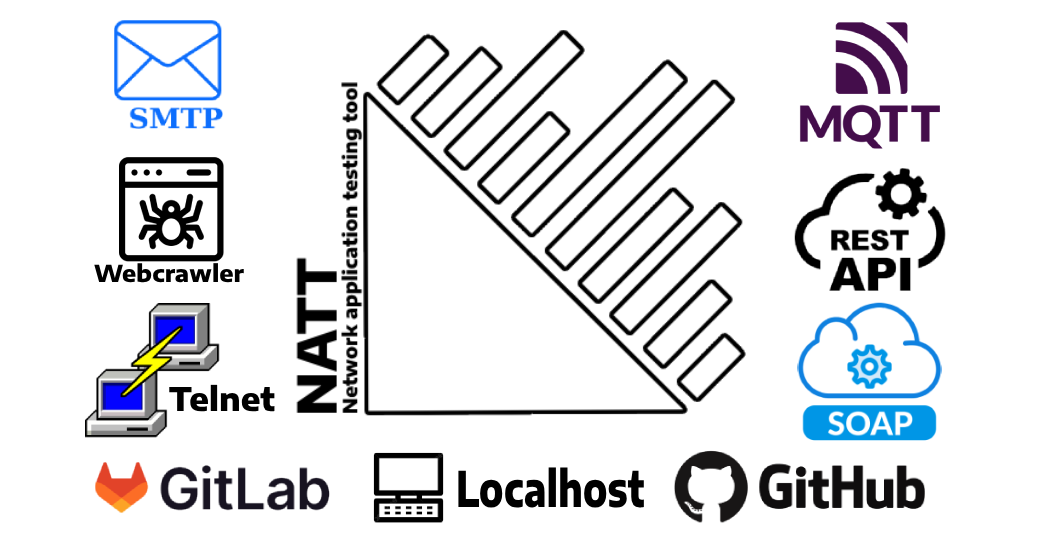
\includegraphics[width=1.0\textwidth]{./imgs/natt-banner-tech.png}
      \caption{Network Application Testing Tool - supported technologies} 
    \end{figure}

  \end{block}

\end{column}

\separatorcolumn

\begin{column}{\colwidth}

  \begin{alertblock}{3. Main features of testing tool}

    This Black Box Testing Tool automates the testing and evaluation of software 
    applications without needing internal implementation details. It supports a 
    wide range of applications, operates independently of external network resources by 
    creating virtual servers and clients, and offers flexible configuration for 
    defining new test scenarios.

    \heading{What does the tool allow you to test?}
    \begin{enumerate}
      \item Testing simple \textbf{email} sending applications
      \item Testing \textbf{clients} that use the telnet protocol
      \item Testing \textbf{servers} that use the telnet protocol
      \item Testing applications that use \textbf{REST API}
      \item Testing \textbf{SOAP web services}
      \item Testing \textbf{MQTT clients}
      \item Testing \textbf{Web crawlers}
      \item Testing the application through the \textbf{standard stream}
    \end{enumerate}

  \end{alertblock}

  \begin{block}{4. Principle of the testing tool}

    Et rutrum ex euismod vel. Pellentesque ultricies, velit in fermentum
    vestibulum, lectus nisi pretium nibh, sit amet aliquam lectus augue vel
    velit. Suspendisse rhoncus massa porttitor augue feugiat molestie. Sed
    molestie ut orci nec malesuada. Sed ultricies feugiat est fringilla
    posuere.

    \begin{figure}
      \centering
        \includegraphics[width=0.3\textwidth]{figures/dag.png}

      \caption{Another figure caption.}
    \end{figure}

  \end{block}

\end{column}

\separatorcolumn

\begin{column}{\colwidth}

  \begin{block}{5. Test scenarios and configuration}

    A different kind of highlighted block.

    $$
    \int_{-\infty}^{\infty} e^{-x^2}\,dx = \sqrt{\pi}
    $$

    Interdum et malesuada fames $\{1, 4, 9, \ldots\}$ ac ante ipsum primis in
    faucibus. Cras eleifend dolor eu nulla suscipit suscipit. Sed lobortis non
    felis id vulputate.

  \end{block}

  \begin{exampleblock}{7. Usage of testing tool}

    Vivamus congue volutpat elit non semper. Praesent molestie nec erat ac
    interdum. In quis suscipit erat. \textbf{Phasellus mauris felis, molestie
    ac pharetra quis}, tempus nec ante. Donec finibus ante vel purus mollis
    fermentum. Sed felis mi, pharetra eget nibh a, feugiat eleifend dolor. Nam
    mollis condimentum purus quis sodales. Nullam eu felis eu nulla eleifend
    bibendum nec eu lorem. Vivamus felis velit, volutpat ut facilisis ac,
    commodo in metus.

  \end{exampleblock}

  \begin{block}{7. Configuration editor}

    Class aptent taciti sociosqu ad litora torquent per conubia nostra, per
    inceptos himenaeos. Phasellus libero enim, gravida sed erat sit amet,
    scelerisque congue diam. Fusce dapibus dui ut augue pulvinar iaculis.

  \end{block}

  \begin{block}{References}

    \nocite{*}
    \footnotesize{\bibliographystyle{plain}\bibliography{poster}}

  \end{block}

\end{column}

\separatorcolumn
\end{columns}
\end{frame}

\end{document}
